\section{Measurements and Results}
\label{sec:Measurements}
A test sample base was created with ten tracks for each class. All of the samples where new samples that were not included in the training sample base.

\subsection{$k$-Means}
The $k$-Means algorithm was used to calculate $k=10$ class centers in our sample base using a batch size of 500 and 50 iterations. These classes were used to classify our test sample base. The tags of the test samples within each class cluster created by the $k$-Means algorithm were counted. The results are shown in figure~\ref{fig:k-Means}. It can be seen that the algorithmically calculated classes do not correspond to the tags defined by our sample base. This was to be expected. Nevertheless it seems that there are some consistent mappings in the structuring of the tags. This needs to be verified by further research.

\begin{figure}[htbp]
\centering
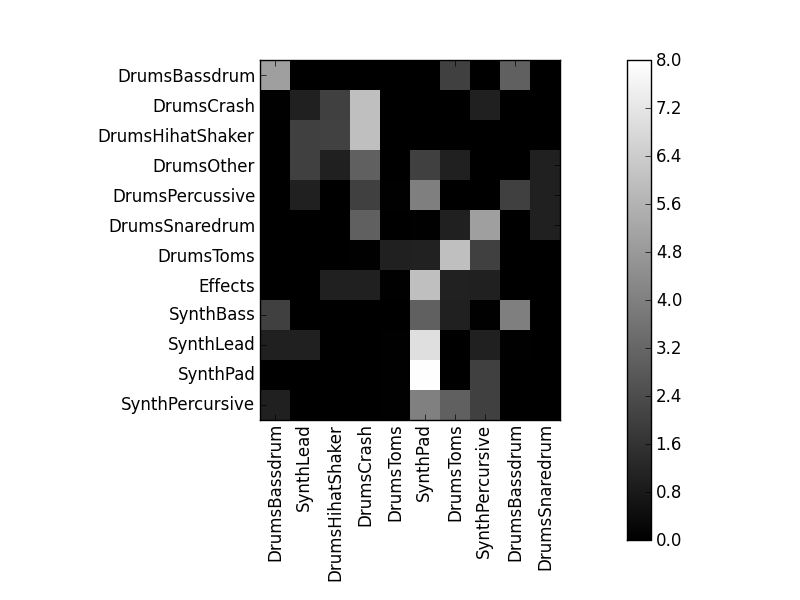
\includegraphics[width=0.45\linewidth]{../plots/k_means_1.png}
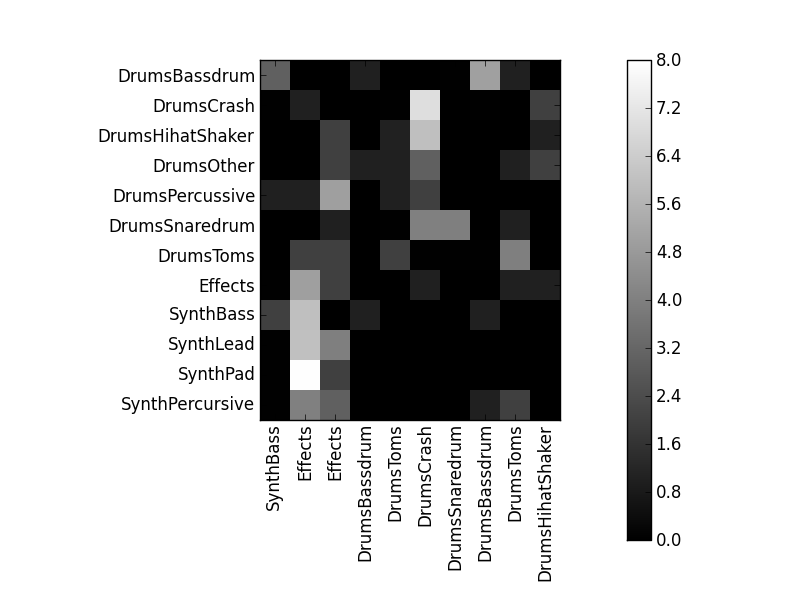
\includegraphics[width=0.45\linewidth]{../plots/k_means_2.png}
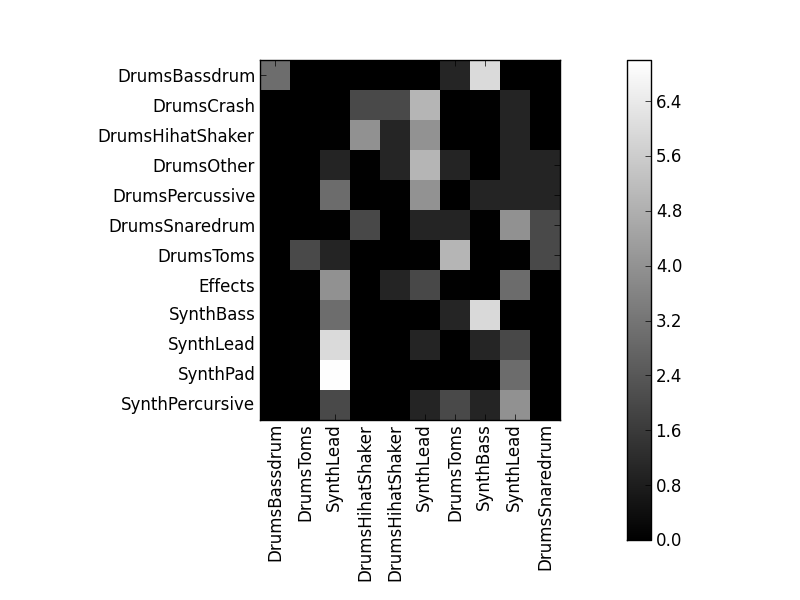
\includegraphics[width=0.45\linewidth]{../plots/k_means_3.png}
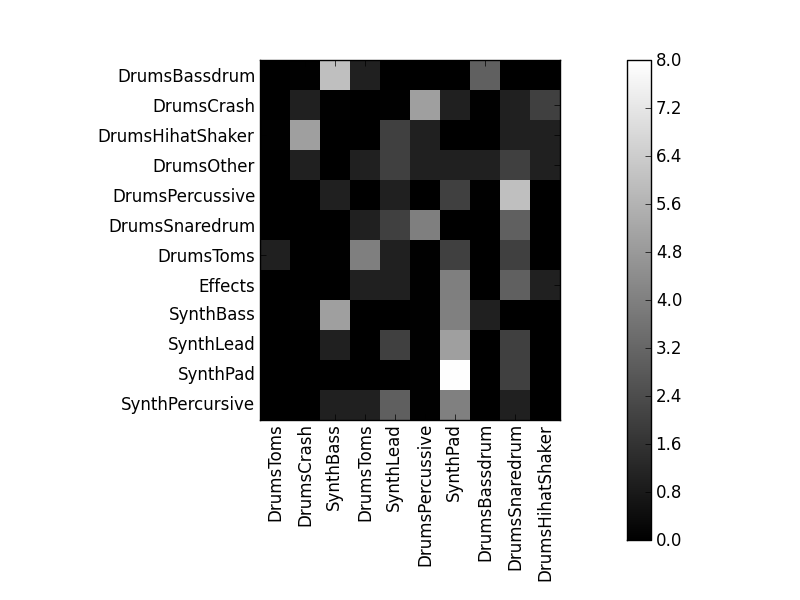
\includegraphics[width=0.45\linewidth]{../plots/k_means_4.png}
\caption{Tagged classes of test samples vs. tags of algorithmically calculated class centers for $k$-Means classification}
\label{fig:k-Means}
\end{figure}

\subsection{$k$-Nearest-Neighbors}
All in the samples of the test sample bank were classified using the implemented $k$-NN algorithm with $k=10$. The results are shown in figure~\ref{fig:k-NN}. The Tags of the test bank are plotted against the tags of the classification. It can be seen that many of the samples are classified correctly. The results overcame our expectations. The variations in the classification correlate with the variances between samples of the same tag in the sample base. This means that the classes which are badly classified are also hard to classify by human perception.

\begin{figure}[htbp]
\centering
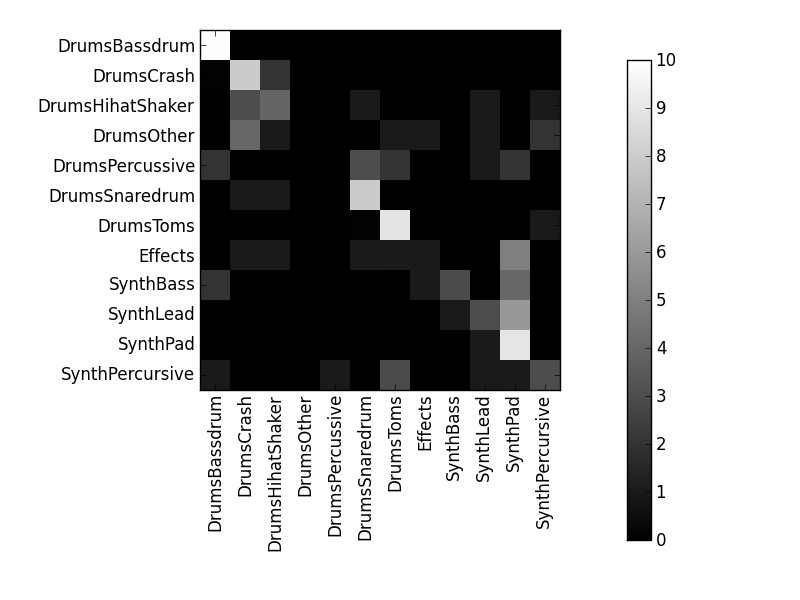
\includegraphics[width=0.45\linewidth]{../plots/knn.png}
\caption{Tagged classes of test samples vs. algorithmically calculated class for $k$-Means classification}
\label{fig:k-NN}
\end{figure}
